\documentclass[b5paper]{standalone} 

\usepackage{tikz}
\usetikzlibrary{intersections,decorations.markings}
\usepackage{commath}

 \pgfmathsetmacro{\delX}{0.7}            %start points, lower left corner
 \pgfmathsetmacro{\delL}{4}
 \pgfmathsetmacro{\delZ}{0.7}


\begin{document}

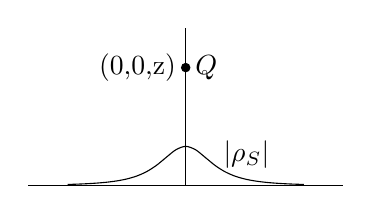
\begin{tikzpicture}
\draw (-2,0)--(2,0);
\draw (0,0)--(0,2);
\draw[fill] (0,1.5) circle (1.5pt);
\draw (0,1.5) node [right]{$Q$}node[left]{(0,0,z)};
%function
\draw[scale=0.5,domain=-3:3,smooth,variable=\x] plot ({\x},{1/sqrt((1+\x*\x)^3)});
\draw (0.8,0.4)node{$\abs{\rho_S}$};
\end{tikzpicture}%

\end{document}
